\documentclass[12pt]{article}
\usepackage[utf8]{inputenc}
\usepackage[spanish]{babel}
\usepackage{amsmath}
\usepackage{amsthm}
\usepackage{array}
\usepackage{multicol,multienum}
\usepackage{graphicx}
\usepackage{float}
\usepackage[autostyle, spanish=mexican]{csquotes}
\usepackage{tikz}
\usepackage{color}
\usepackage{anysize}
\usepackage{anyfontsize}
\usepackage{siunitx}
\usepackage{minted}
\usepackage[minted,xparse,breakable]{tcolorbox}
\usepackage[os=win]{menukeys}
%Este paquete permite manejar los encabezados del documento
\usepackage{fancyhdr}
%hay que definir el ambiente de la página
\pagestyle{fancy}
\fancyhf{}
%\fancyheadoffset{0.05\textwidth}
%aqui va el texto para todas las paginas l--> izquierda, r--> derecha, hay un C--> para centrar el texto deseado
%\lhead{Curso de Física Computacional}
\fancyhead[L]{\nouppercase{\leftmark}}
\fancyhead[R]{\nouppercase{\rightmark}}
\fancyfoot[C]{\thepage}

%define el ancho de la linea que separa el encabezado del cuerpo del texto
\renewcommand{\headrulewidth}{0.5pt}
\setlength{\parskip}{1em}
\renewcommand{\baselinestretch}{1.5}
\interfootnotelinepenalty=8000
\usepackage{hyperref}
%esta parte define el color del marco que aparece en las hiperreferencias.
\definecolor{links}{HTML}{2A1B81}
\hypersetup{colorlinks,linkcolor=,urlcolor=links}
\newcommand{\azulfuerte}[1]{\textcolor{blue}{\textbf{#1}}}
\spanishdecimal{.}
%\marginsize{1.5cm}{1.5cm}{1.5cm}{1.5cm}
\newcommand{\python}{\texttt{python}}
%\usepackage{courier}
\usepackage{listingsutf8}
\usepackage{listings}
\usepackage{xcolor}
\usepackage{textcomp}
\usepackage{color}
\definecolor{deepblue}{rgb}{0,0,0.5}
\definecolor{brown}{rgb}{0.59, 0.29, 0.0}
\definecolor{OliveGreen}{rgb}{0,0.25,0}
% \usepackage{minted}

\DeclareCaptionFont{white}{\color{white}}
\DeclareCaptionFormat{listing}{\colorbox{gray}{\parbox{0.98\textwidth}{#1#2#3}}}
\captionsetup[lstlisting]{format=listing,labelfont=white,textfont=white}
\renewcommand{\lstlistingname}{Código}


\definecolor{Code}{rgb}{0,0,0}
\definecolor{Keywords}{rgb}{255,0,0}
\definecolor{Strings}{rgb}{255,0,255}
\definecolor{Comments}{rgb}{0,0,255}
\definecolor{Numbers}{rgb}{255,128,0}

\makeatletter

\newif\iffirstchar\firstchartrue
\newif\ifstartedbyadigit
\newif\ifprecededbyequalsign

\newcommand\processletter
{%
  \ifnum\lst@mode=\lst@Pmode%
    \iffirstchar%
        \global\startedbyadigitfalse%
      \fi
      \global\firstcharfalse%
    \fi
}

\newcommand\processdigit
{%
  \ifnum\lst@mode=\lst@Pmode%
      \iffirstchar%
        \global\startedbyadigittrue%
      \fi
      \global\firstcharfalse%
  \fi
}

\lst@AddToHook{OutputOther}%
{%
  \lst@IfLastOtherOneOf{=}
    {\global\precededbyequalsigntrue}
    {}%
}

\lst@AddToHook{Output}%
{%
  \ifprecededbyequalsign%
      \ifstartedbyadigit%
        \def\lst@thestyle{\color{orange}}%
      \fi
    \fi
  \global\firstchartrue%
  \global\startedbyadigitfalse%
  \global\precededbyequalsignfalse%
}

\lstset{ 
language=Python,                % choose the language of the code
basicstyle=\footnotesize\ttfamily,       % the size of the fonts that are used for the code
numbers=left,                   % where to put the line-numbers
numberstyle=\scriptsize,      % the size of the fonts that are used for the line-numbers
stepnumber=1,                   % the step between two line-numbers. If it is 1 each line will be numbered
numbersep=5pt,                  % how far the line-numbers are from the code
backgroundcolor=\color{white},  % choose the background color. You must add \usepackage{color}
showspaces=false,               % show spaces adding particular underscores
showstringspaces=false,         % underline spaces within strings
showtabs=false,                 % show tabs within strings adding particular underscores
frame=single,   		% adds a frame around the code
tabsize=2,  		% sets default tabsize to 2 spaces
captionpos=t,   		% sets the caption-position to bottom
breaklines=true,    	% sets automatic line breaking
breakatwhitespace=false,    % sets if automatic breaks should only happen at whitespace
escapeinside={\#},  % if you want to add a comment within your code
stringstyle =\color{OliveGreen},
%otherkeywords={{as}},             % Add keywords here
keywordstyle = \color{blue},
commentstyle = \color{black},
identifierstyle = \color{black},
literate=%
         {á}{{\'a}}1
         {é}{{\'e}}1
         {í}{{\'i}}1
         {ó}{{\'o}}1
         {ú}{{\'u}}1
%
%keywordstyle=\ttb\color{deepblue}
%fancyvrb = true,
}

\lstdefinestyle{FormattedNumber}{%
    literate={0}{{\textcolor{red}{0}}}{1}%
             {1}{{\textcolor{red}{1}}}{1}%
             {2}{{\textcolor{red}{2}}}{1}%
             {3}{{\textcolor{red}{3}}}{1}%
             {4}{{\textcolor{red}{4}}}{1}%
             {5}{{\textcolor{red}{5}}}{1}%
             {6}{{\textcolor{red}{6}}}{1}%
             {7}{{\textcolor{red}{7}}}{1}%
             {8}{{\textcolor{red}{8}}}{1}%
             {9}{{\textcolor{red}{9}}}{1}%
             {.0}{{\textcolor{red}{.0}}}{2}% Following is to ensure that only periods
             {.1}{{\textcolor{red}{.1}}}{2}% followed by a digit are changed.
             {.2}{{\textcolor{red}{.2}}}{2}%
             {.3}{{\textcolor{red}{.3}}}{2}%
             {.4}{{\textcolor{red}{.4}}}{2}%
             {.5}{{\textcolor{red}{.5}}}{2}%
             {.6}{{\textcolor{red}{.6}}}{2}%
             {.7}{{\textcolor{red}{.7}}}{2}%
             {.8}{{\textcolor{red}{.8}}}{2}%
             {.9}{{\textcolor{red}{.9}}}{2}%
             {\ }{{ }}{1}% handle the space
         ,%
          %mathescape=true
          escapeinside={__}
          }



\author{M. en C. Gustavo Contreras Mayén.}
\title{Manejo de archivos de datos con \python \\ \begin{Large} Curso de Física Computacional\end{Large} \\
\begin{small}
\texttt{curso.fisica.comp@gmail.com}
\end{small}}
\date{ }
\begin{document}
\maketitle
\fontsize{14}{14}\selectfont
\section{Los archivos de datos con \python.}
\subsection{Consideraciones}
Una tarea muy común y frecuente en el ámbito de la Física Computacional, será el manejo de archivos de datos para su proceso y análisis.
\par
Como una primera tarea que hay que atender en el desarrollo de prácticas de programación bajo cualquier lenguaje, es la generación de un archivo de datos con una serie de características necesarias:
\begin{enumerate}
\item Una estructura de construcción, que permita la posterior lectura del archivo.
\item La codificación de los caracteres que conforman los datos, este punto es crítico si además de números, se incluyen o manejan cadenas de texto (el manejo de acentos y ciertos caracteres es crítico si no se considera este elemento)
\end{enumerate}
\subsection{Estructura del archivo.}
Debemos de elegir anticipadamente el tipo de archivo que vamos a generar, ya que de esta forma, al momento de definir el código, se implementará la estructura del archivo.
\par
Quien reciba el archivo para su procesamiento, análisis, etc. debe de conocer el tipo de estructura que lleva. En el posible caso de que no avisemos esta información, el usuario del archivo, deberá de hacer una revisión preliminar del archivo para identificar la estrucutura. En el caso de que nosotros seamos los usuarios de un archivo de datos y no tengamos la informción, será nuestra tarea entonces, hacer la revisión de la estructura interna del archivo.
\par
Existen diversos formatos para los archivos de texto, a continuación se describen cuatro de los más conocidos:
\begin{table}[H]
\centering
\begin{tabular}{| m{3.5cm} | m{10cm} |}
\hline
\textbf{Tipo de archivo} & \multicolumn{1}{>{\centering\arraybackslash} m{10cm}|}{\textbf{Descripción}} \\ \hline
txt & Texto plano que representa sólo caracteres (o cadenas), excluye cualquier tipo de metadatos. \\ \hline
csv & Valores separados por coma (Comma-separated values), utiliza comas (u otro delimitador) para estructurar los datos almacenados, permitiendo guardarlos en un formato tipo tabla. \\ \hline
HMTL & Lenguaje de marcado de hipertexto (HyperText Markup Language) almacena los datos de manera estrucutrada, se utiliza comúnmente en páginas web. \\ \hline
JSON  & Notación de objeto de JavaScript (JavaScript Object Notation) es un formato sencillo y eficiente, siendo un formato para almacenar y transferir datos. \\ \hline
\end{tabular}
\end{table}
Al momento en que compartan el archivo, se recomienda elaborar un archivo \textbf{README}, que contiene información acerca de otros archivos ya sea en un directorio o un archivo comprimido.
\par
Es una forma de documentación de software, consiste en un archivo de texto plano llamado \textbf{READ.ME}, \textbf{README.TXT}, \textbf{README.md} (para un archivo markdown), \textbf{README.1ST} o simplemente \textbf{README}.
\par
El nombre del archivo es generalmente escrito en mayúsculas. En los sistemas Unix-like, generalmente los nombres se escriben en minúscula, y esto hace que en un listado de archivos salga primero el archivo \textbf{README}.
\section{Creando un archivo de datos.}
Con \python\ será una tarea muy frecuente el generar un archivo de datos y compartirlo con otros usuarios.
\par
Las instrucciones para crear el archivo son sencillas de implementar en el código, toma en cuenta lo siguiente:
\begin{enumerate}
\item El archivo de datos se va a crear en la misma carpeta en donde se está ejecutando el archivo de \python, es decir, el archivo con extensión \texttt{*.py}.
\item Es posible tanto la escritura como la lectura de archivos que estén ubicados en otro directorio que no sea en donde se ejecuta el archivo de \python, que involucra el manejo de paquetes, módulos y funciones para el uso del sistema operativo, rutas relativas, etc., pero en esta revisión nos enfocamos al trabajo de los archivos de texto en la misma carpeta del archivo que se ejecuta.
\item Un archivo de datos requiere de la \enquote{apertura} de un espacio en memoria, para que con una instrucción, se \enquote{escriban} los datos en el archivo.
\item Una vez que se completa la tarea de escribir los datos, hay que cerrar el espacio de memoria.
\end{enumerate}
\newpage
\section{Crear un archivo de datos}
Un objeto de tipo \texttt{file} se crea cuando se abre un archivo donde se requiere tanto un \texttt{nombre}, así como un \texttt{modo}.
\par
El \texttt{nombre} del archivo puede referirse como una ruta absoluta o como un ruta relativa en el directorio donde se está ejecutando el archivo de \texttt{pyhton}. Por ejemplo, para abrir un archivo en modo de \emph{escritura}, la sintaxis sería la siguiente

\mint{python}|archivo = open('nombrearchivo.txt', 'w')|

Los objetos \mintinline{python}|file| se deben de cerrar con el método \mintinline{python}|close|, en el ejemplo anterior sería: \mintinline{python}|archivo.close()|.
\par
Cuando un programa termina o se interrumpe, \python{} cierra automáticamente cualquier objeto \mintinline{python}|file|.
\par
En la siguiente tabla se muestran los modos para los objetos de tipo \mintinline{python}|file|:
\begin{table}[H]
\begin{tabular}{| m{2cm} | m{12cm} |}
\hline
\texttt{mode} & Modo de apertura \\ \hline
\texttt{r} & Texto, De solo lectura (modo por defecto) \\ \hline
\texttt{w} & Texto, escritura (Si el archivo no existe, se crea. Si el archivo existe, se sobre escribe) \\ \hline
\texttt{a} & Texto, Se agrega contenido al archivo que ya existe \\ \hline
\texttt{r+} & Texto, De lectura y escritura \\ \hline
\end{tabular}
\end{table}
Cabe señalar que existen otros cuatro modos para un archivo, pero cuando éste es un archivo \emph{binario}, es decir, la información que contiene el archivo está codificada en binario (unos y ceros). En el curso de Física Computacional \textbf{siempre} usaremos archivos de texto.
\section{Escribiendo los datos}
Haremos una revisión de la técnica para escribir datos en un archivo de texto plano, considera que se hace énfasis en que trabajaremos con datos obtenidos de algún algoritmo del curso de Física Computacional; el manejo de archivos de \emph{entrada y salida} es en sí, un tema que requiere de mayor atención y tiempo para un manejo más completo, pero con esta revisión, tendremos lo necesario para generar archivos de datos.
\subsection{Uso de la instrucción \texttt{print}}
Ya hemos trabajado con una función de salida que nos permite visualizar los datos en la terminal, ésta es la función \mintinline{python}|print()|, al agregar un parámetro adicional a esta función se puede incluir esos datos en un archivo, en el ejemplo a partir de una secuencia de enteros del $1$ al $99$:
\begin{minted}[linenos=True]{Python}
archivo01 = open('potencias01.txt', 'w')
for i in range(1, 100):
    print(i, i**2, i**3, i**4, sep=',', file=archivo01)
archivo01.close()    
\end{minted}
Veamos lo que ocurre en este código:
\begin{enumerate}
\item En la línea $1$ ocupamos una variable \mintinline{python}{archivo01} que hace referencia al archivo de texto \mintinline{python}{potencias01.txt}. Considera que es posible utilizar libremente otras extensiones al archivo de datos: \emph{*.dat}, \emph{*.inf}, \emph{*.text}, \emph{*.data}, etc.
\par
Lo relevante de la extensión es que el sistema operativo con el que trabajen, pueda distinguir que se trata de un archivo de datos en texto plano.
\par
Como segundo argumento, se indica la \textit{'w'} como parámetro de la función, esto indica que se va a realizar la instrucción \textit{write}, lo que permitirá escribir en el archivo. Como punto importante volvemos a señalar que en caso de que el archivo \textit{potencias01.txt} no exista, \python\ creará un archivo nuevo, en caso de que ya exista, lo va a sobre-escribir.
\item En la línea $2$ creamos nuestra secuencia de enteros, mediante la función \mintinline{python}{range(1, 100)}.
\item En la línea $3$ se incorporan dos nuevos parámetros para la función \mintinline{python}{print}: \mintinline{python}{sep=','} que nos indica que el \emph{separador} entre los datos, será en este caso una coma. Es posible utilizar otros separadores, como el espacio en blanco (que es el valor por defecto) o un tabulador, este separador es muy importante ya que debemos de considerarlo cuando se haga la operación de lectura de los datos del archivo.
\par
El siguiente parámetro es la asignación \mintinline{python}{file=archivo01} que corresponde a la asignación de la variable de tipo \texttt{file}, al argumento de la función \texttt{print}.
\item En la línea $4$, se cierra el objeto \texttt{file} mediante la función \texttt{close()}.
\end{enumerate}
Al abrir el archivo \texttt{potencias01.txt} con un editor de texto, veremos los valores correspndientes a las potencias, siendo una coma el separador entre ellos, nótese que no hay un espacio en blanco entre los valores.
\subsection{Con el método \texttt{write}}
La siguiente manera con la que podemos crear un archivo de datos, es usando el método \mintinline{python}{write()}, que nos permite establecer un formato en la cadena que lleva como argumento:
\begin{minted}[breaklines, linenos=True]{Python}
archivo02 = open('potencias02.txt', 'w')
for i in range(1, 100):
    archivo02.write('{0:} \t {1:} \t {2:} \t {3:} \n'.format(i, i**2, i**3, i**4))
archivo02.close()
\end{minted}
En donde en la línea $3$, vemos que el formato para la cadena es el que ya hemos ocupado previamente en el curso; se utiliza una tabulación como separador entre las columnas.
\par
Luego de la cuarta referencia en la cadena, se ha incluido un salto de línea \texttt{\textbackslash n}, con esto se coloca un nuevo renglón en el archivo de datos para almacenar los valores de la siguente iteración, en caso de no incorporar ese salto de línea, se tendría un único renglón con todos los datos, lo que nos dificultaría su lectura en un siguiente paso.
\subsection{Usando \texttt{numpy.savetxt}}
Del paquete \mintinline{python}{numpy} contamos con un conjunto de funciones que nos permitirán el manejo más directo para guardar archivos.
\par
Con la función \mintinline{python}{savetxt}, se simplifica el código ya que no se requiere la creación previa del archivo de datos, como veremos en el siguiente ejemplo
\begin{minted}[linenos=True]{Python}
import numpy as np

x = []
y = []
z = []
for i in range(1, 100):
    x.append(i)
    y.append(i**2)
    z.append(i**3)

np.savetxt('potencias03.txt', (x, y, z), delimiter=',')
\end{minted}
El ejercicio sigue siendo el mismo: calcular las potencias de los enteros del $1$ al $99$, pero ahora se hace con un modo más \emph{pythónico}, es decir, con las instrucciones propias del lenguaje.
\par
Definimos tres listas vacías $x, y z$ para almacenar los valores de las operaciones que se realizan dentro del ciclo \mintinline{python}{for}, el método \mintinline{python}{savetxt} requiere el nombre del archivo de datos (\emph{potencias03.txt}), así como el delimitador (\texttt{delimiter=','}).
\par
Cuando ejecutamos el código y revisamos el contenido del archivo de datos, encontramos que los valores se han agregado de la siguiente manera y formato:
\begin{minted}{Python}
1.000000000000000000e+00,2.000000000000000000e+00,3.00...000e+00,...
1.000000000000000000e+00,4.000000000000000000e+00,9.00...000e+00,...
1.000000000000000000e+00,8.000000000000000000e+00,2.70...000e+01,...
\end{minted}
Es decir, tenemos un arreglo por cada renglón y además cada valor con un formato de notación científica. ¿Cómo podríamos mejorar el resultado del conjunto de datos?
\par
\textcolor{blue}{Respuesta:} Usando \mintinline{python}{numpy} al modificar la siguiente línea del código
\mint[breaklines]{Python}{np.savetxt('potencias03.txt',np.transpose([x, y, z]), delimiter=',', fmt='%d')}
donde hacemos la transpuesta de la lista de listas; con el argumento \texttt{fmt='\%d'} modificamos el formato a un tipo entero, entiendo entonces que el formato visto en la primera ejecución es el formato por defecto: \texttt{fmt='\%.18e'}
\par
En el siguiente ejemplo ocupando nuevamente \mintinline{python}{savetxt}, veremos que podemos guardar en un archivo un objeto de \mintinline{python}{numpy}:
\begin{minted}[linenos=True]{Python}
x = np.array([[1, 2, 3], 
[4, 5, 6],
[7, 8, 9]], np.int32)

np.savetxt("test.txt", x)
np.savetxt("test2.txt", x, fmt="%2.3f", delimiter=",")
np.savetxt("test3.txt", x, fmt="%04d", delimiter=" :-) ")
\end{minted}
Donde se han modificado el formato y el tipo de delimitador entre los valores.
\subsection{Incluyendo cabeceras en el archivo}
Hemos visto la manera en la que ya podemos almacenar un conjunto de datos que se generan a partir de un algoritmo en \python, pero pensando en que debemos de ser lo más claros posibles al momento de que esos archivos de datos se compartan, es preciso que se incluyan \emph{cabeceras} que identifiquen de algún modo cada columna dentro del archivo.
\par
Las cabeceras suelen ser referencias a letras o palabras que permitan reconocer lo que almacena esa columna. Ya hemos trabajado con cabeceras para visualizar en la terminal un conjunto de datos:
\begin{minted}{Python}
x        exacta            suma           error
1        0.3894183423    0.3893333333    2.18297e-02
2        0.3894183423    0.3894186667    8.32929e-05
3        0.3894183423    0.3894183416    1.85238e-07
\end{minted}
Mientras que un comentario es una línea de código que inicia con el carácter \texttt{\#}, seguido de una cadena que proporciona información al respecto. El uso de los comentarios es oportuno, pero veremos más adelante que al momento de leer un archivo, suele requerir un ajuste para que no se lea ese renglón.
\par
Veamos el siguiente ejemplo que incorpora comentarios y cabeceras:
\begin{minted}[breaklines, linenos=True]{Python}
t = np.arange(0.1, 30., 0.5)
d = np.arange(0.1, 60., 1)

comentario1 ='# Este es un comentario sobre el archivo'
comentario2 = '# Sirve de ejemplo para diferenciar un comentario de una cabecera'
cabecera = 'Tiempo \t Velocidad'

with open('potencias05.txt', 'a') as f1:
    f1.write(comentario1 + '\n')
    f1.write(comentario2 + '\n')
    f1.write(cabecera + '\n')
    f1.close()
    
with open('potencias05.txt', 'a') as f2:
    for i in range(len(t)):
        v = d[i]/t[i] 
        f2.write('{0:} \t {1:1.4f} \n'.format(i, v))
    f2.close()
\end{minted}
En el código se ha utilizado la instrucción \mintinline{python}{with}, que permite el manejo del tipo de objeto \mintinline{python}{file} de una manera mucho más oportuna, es decir, mediante el alias \texttt{as} tenemos el control en todo momento desde que se inicializa el objeto, se trabaja con él y se cierra.
\par
El modo del archivo de datos se modificó a \emph{append}, es decir: \texttt{'a'}, con ello, se podrá agregar contenido al archivo, recuerda que si el archivo no existe, se crea. Pero ten cuidado con su manejo, ya que si ejecutas nuevamente el código, se va a agregar todo el contenido nuevamente.
\par
En el archivo de datos tendremos lo siguiente
\begin{minted}[breaklines]{Python}
#Este es un comentario sobre el archivo
#Sirve de ejemplo para diferenciar un comentario de una cabecera
Tiempo 	 Velocidad
0 	 1.0000 
1 	 1.8333 
2 	 1.9091 
3 	 1.9375 
\end{minted}
\section{Recuperando los datos}
\subsection{Usando numpy}
Una vez que ya tenemos un archivo de datos, el siguiente paso es recuperar el conjunto de información dentro del mismo, recordemos que hemos mencionado que si contamos con un archivo \textbf{READ.ME}, tendremos una referencia sobre lo que viene dentro del archivo, o esperamos al menos que contenga comentarios y cabeceras de información.
\par
Nos enfocaremos al uso del paquete \mintinline{python}{numpy} para la lectura de datos, cabe aclarar que con el manejo de archivos de tipo \texttt{*.csv}, se requiere de un manejo más a detalle, ya que estos archivos normalmente se obtienen de hojas de cálculo, como Excel o Calc de LibreOffice.
\subsection{La función \texttt{loadtxt}}
Ahora ocuparemos el archivo \texttt{potencias05.txt} que generamos en la sección anterior, recordemos que el archivo \emph{debe de estar en el mismo directorio} de nuestro programa ejecutable. La sintaxis de la función es:
\begin{minted}[breaklines]{Python}
import numpy as np

datos = np.loadtxt('potencias05.txt', delimiter='\t', skiprows=3)

tiempo = datos[:,0]
velocidad = datos[:,1]

print(tiempo)
print(velocidad)
\end{minted}
El argumento \texttt{skiprows=3} no incluye las tres primeras líneas del archivo, que es en donde están los comentarios y la cabecera, por lo que tenemos solo los datos en un arreglo por cada columna. Usando el \emph{slicing}, seleccionamos mediante un índice el contenido para cada columna, recordemos que en \python, los índice comienzan en cero. De esta manera contamos con las columnas del archivo de datos en arreglos independientes y con ellos ya podremos operarlos, graficarlos, etc.
\par
Dentro de la documentación oficial de \python, puedes revisar más a profundidad este tema y con ello extender su manejo para que puedas ocupar archivos de datos y reforzar tus códigos durante el curso de Física Computacional.
% \subsection{El código con \python.}
% Del ejercicio que se realizó para resolver el cálculo de valores a través de la interpolación de Newton:
% \begin{minted}[breaklines, linenos=True]{Python}
% from newtonPoli import coeficientes, evaluaPoli
% import numpy as np

% resultados = open('DatosNewton.dat','w')

% xDatos = np.array([0.15,2.30,3.15,4.85,6.25,7.95])
% yDatos = np.array([4.79867,4.49013,4.2243,3.47313,2.66674,1.51909])

% a = coeficientes(xDatos, yDatos)

% print ('{:^3} \t {:^7} \t {:^7} \t {:<11}'.format('x', 'yInterpol', 'yExacta', 'Err relativo'))
% print ('-'*55)


% for x in np.arange(0.0, 8.1, 0.5):
%     y = evaluaPoli(a, xDatos, x)
%     yExacta = 4.8 * np.cos(np.pi*x/20.0)
%     print ('{:1.1f} \t {:1.5f} \t {:1.5f} \t {:1.5E}'.format(x, y, yExacta, abs(yExacta - y)/yExacta*100))
%     resultados.write ('{:1.1f} \t {:1.5f} \t {:1.5f} \n'.format(x, y, yExacta))
    
% resultados.close()
% \end{minted}
% En la línea 4 del código, se indica la función \azulfuerte{open}, que se requiere para \enquote{abrir} el espacio para el archivo, recibe como primer argumento el nombre del archivo y su extensión: \emph{DatosNewton.dat}, nótese que la extensión que hemos dejado, es \emph{*.dat}, se puede utilizar libremente el tipo de extensión \emph{*.txt}, \emph{*.inf}, \emph{*.text}, \emph{*.data}, etc.
% \par
% Lo relevante de la extensión es que el sistema operativo con el que trabajen, pueda distinguir que se trata de un archivo de datos en texto plano.
% \par
% Como segundo argumento, se indica la \textit{'w'} en la misma línea 4 del código, indica que se va a realizar la instrucción \textit{write}, lo que permitirá escribir en el archivo. Como punto importante hay que señalar, que en caso de que el archivo \textit{DatosNewton.dat} no exista, \python\ creará un archivo nuevo, en caso de que ya exista, lo va a sobre-escribir.
% \par
% En la línea 19 del código, se señala la instrucción que va a escribir los datos en el archivo: \texttt{resultados.write(argumento)}, en donde en el caso del ejercicio, el argumento consiste en una cadena de formato para tres columnas, cada una de ellas, separada mediante una tabulación (\texttt{\textbackslash t}) y al final de la cadena de formato, se incluye un salto de línea (\textbackslash n), que permitirá que en el siguiente ciclo del bucle, se escriba en otra línea del archivo, los valores que se calculan en esa iteración.
% \par
% Una vez concluido el proceso de iteración, o el proceso donde se calcularon los valores del problema, se debe de cerrar el espacio del archivo, o de lo contrario tendremos un error. Para cerrar el objeto tipo \emph{file}, se ocupa la función \azulfuerte{nombreobjeto.close()}, como lo vemos en la línea de código 21.
% \par
% Con estas instrucciones de manejo de un archivo, ya contamos en nuestro directorio de un archivo de datos que podremos utilizar posteriormente. Toma en cuenta que no se han incluido cabeceras de las columnas, en el ejercicio, las líneas 11 y 12, muestran en la terminal una cabecera con el nombre de la columna y una línea que separa a modo de tabla.
% \par
% La pregunta natural es: ¿podremos incluir cabeceras o información adicional en nuestro archivo y que no interfiera con la recuperación de los datos?
% \section{Recuperando los datos.}
% Siguiendo con el ejercicio de la interpolación de Newton y contando ya con un archivo de datos: \emph{DatosNewton.dat}, ahora nos aplicaremos para recuperar los datos y con ellos, generar una gráfica con la librería \azulfuerte{\texttt{matplotlib}}.
% \subsection{Extraer los datos del archivo.}
% Revisemos el código que se requiere para primero obtener los datos del archivo y posteriomente usar la rutina ya conocida para graficar.
% \begin{lstlisting}[style= FormattedNumber, basicstyle=\linespread{1.1}\ttfamily=\normal, columns=fullflexible]
% import matplotlib.pyplot as plt
% import csv

% x = []
% yi = []
% ye = []


% with open('DatosNewton.dat', 'r') as csvfile:
%     plots = csv.reader(csvfile, delimiter = '\t')
%     for row in plots:
%        x.append(float(row[0]))
%        yi.append(float(row[1]))
%        ye.append(float(row[2]))
       

% plt.plot(x, yi, label='Polinomio Newton', ls = 'dashed')
% plt.plot(x, ye, label='Valor exacto', color = 'red')
% plt.title('Grafica de los datos de un archivo')
% plt.legend(loc = 1)
% plt.show()
% \end{lstlisting}
% En la línea 2 se importa la librería \emph{csv} que permitirá el manejo de un archivo de este tipo; como se mencionó en el apartado anterior, se requiere conocer el tipo de delimitador que se utilizó para generar el archivo.
% \par
% Se requieren tres listas en donde vamos a almacenar los valores del archivo:
% \begin{enumerate}
% \item Un arreglo para representar la variable independiente, en este caso $x$.
% \item Un arreglo para los valores de interpolación $yi$.
% \item Un arreglo para los valores evaluados con la función exacta $ye$.
% \end{enumerate}
% En la línea 9 del código mediante la instrucción \azulfuerte{\texttt{with open}}, se declara un objeto de tipo \texttt{file}, al que se le da un alias: \texttt{csvfile}. Necesita al menos de dos argumentos: el nombre del archivo y el tipo de operación que se va a ejecutar, en nuestro ejemplo, vamos a usar \texttt{r}, que corresponde a la acción de leer los datos del archivo. Toma en cuenta que con la misma función \azulfuerte{\texttt{open}}	se pueden realizar las tareas de escribir un archivo y de leer los datos contenidos en el mismo.
% \par
% Una vez definido el objeto \texttt{file}, se necesita recuperar los elementos contenidos, para ello usamos la función \azulfuerte{\texttt{csv.reader}}, con dos argumentos: el nombre del objeto file y el delimitador con el que se guardó el archivo. El delimitador es un argumento necesario, como se mencionó previamente para los archivos de datos, puede usar un delimitador:
% \begin{itemize}
% \item Espacio en blanco.
% \item Tabulación.
% \item Coma.
% \item Guión.
% \end{itemize}
% De acuerdo al delimitador utilizado, se debe de indicar en el respectivo argumento, para nuestro ejemplo \texttt{delimiter = $'\backslash t'$}.
% \subsection{Almacenando temporalmente los datos.}
% Posteriormente tenemos un ciclo \azulfuerte{\texttt{for}}, mediante el cual se van agregando los elementos del archivo en cada lista, toma en cuenta que los datos que están en el archivo, a pesar de que la representación que vemos de ellos, correspondan a números, \python\ los guardó como \textbf{\texttt{strings}}, siendo necesario la conversión a un tipo de dato \textbf{float} para su uso en la gráfica.
% \par
% A partir de la línea 17 del código, se presenta la rutina de graficación ya conocida y manejada en el curso de Física Computacional.
% \par
% El resultado obtenido es la siguiente gráfica:
% \begin{figure}[H]
% \centering
% 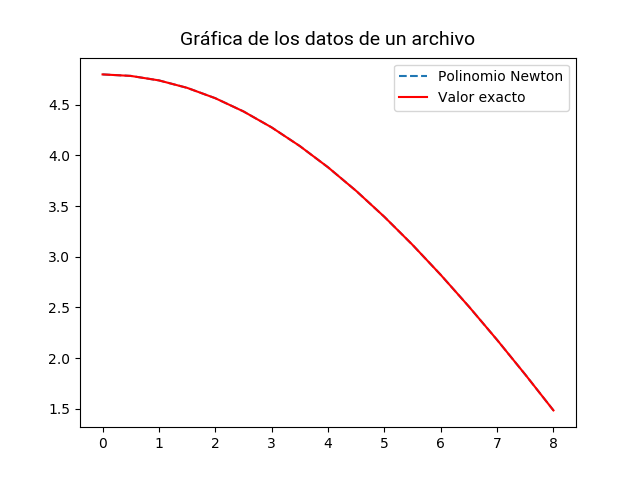
\includegraphics[scale=0.9]{Imagenes/Archivos_01}
% \caption{Gráfica generada a partir de los datos en un archivo.}
% \end{figure}
% Las opciones que hemos visto para el manejo de archivos son las básicas, podrás extender su uso e implementación cuando revises la respectiva documentación.
% \par
% El potencial que se tiene con \python\ para el manejo de arhivos es muy grande, ya que se pueden manejar archivos de datos y analizarlos sin necesidad de cambiar de formatos, por ejemplo, un archivo de datos en Excel (que en algunos casos suele ser un tipo de archivo aceptado para el ámbito científico) se puede operar con librerías especializadas como \texttt{\textbf{pandas}} que contiene funciones que operan directamente en los archivos.
\end{document} 